
%(BEGIN_QUESTION)
% Copyright 2007, Tony R. Kuphaldt, released under the Creative Commons Attribution License (v 1.0)
% This means you may do almost anything with this work of mine, so long as you give me proper credit

When considering the propagation of high-frequency electrical signals along a pair of conductors, it is important to remember that all cables possess distributed {\it capacitance} and {\it inductance} along their length:

$$\includegraphics[width=15.5cm]{i02180x01.eps}$$

This means every electrical cable has the ability to store energy, in both an electric field (in the capacitance) and a magnetic field (in the inductance).  This has profound impact on how high-frequency and transient (pulse) signals ``see'' the cable.  No longer can we view a cable as a simple pair of wires, but it must now be considered a component in its own right.

\vskip 10pt

Examining the cable model comprised of multiple capacitors and inductors in a series/parallel arrangement, try to determine voltages and currents along the cable immediately after the output of the digital logic gate goes from a ``low'' state to a ``high'' state:

$$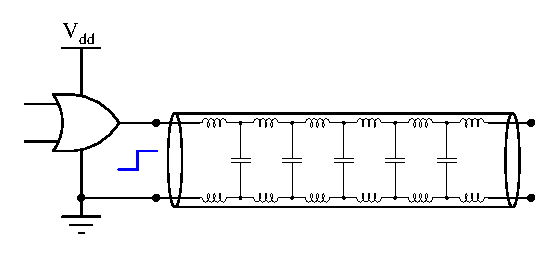
\includegraphics[width=15.5cm]{i02180x02.eps}$$

\underbar{file i02180}
%(END_QUESTION)





%(BEGIN_ANSWER)

The cable will draw current from the gate output as the capacitances and inductances ``charge,'' then the current will stop and the cable will act as an open.  This charging time primarily depends on the length of the cable.

\vskip 10pt

Challenge question: what factor or factors determine the amount of current drawn from the gate as it ``powers'' the cable?

%(END_ANSWER)





%(BEGIN_NOTES)

Cable geometry determines surge impedance, which then determines current draw according to Ohm's Law ($I = {V \over R}$).

%INDEX% Electronics review: characteristic impedance of transmission line
%INDEX% Electronics review: surge impedance of transmission line

%(END_NOTES)


